Hier soll nun ein Verfahren hergeleitet und anschließend mit zwei vereinfachten Verfahren verglichen werden. 

Für die Erzeugung der Isolationsspektren wird hier das System um den Isolator erweitert und als Zweimassenschwinger (\cref{fig:vkm}) betrachtet, wobei der obere Schwinger die aufgehende Struktur (1) und der untere Schwinger den Isolator (2) samt des steifen Kellergeschosses beschreiben soll.

\begin{figure}[ht]
    \centering
    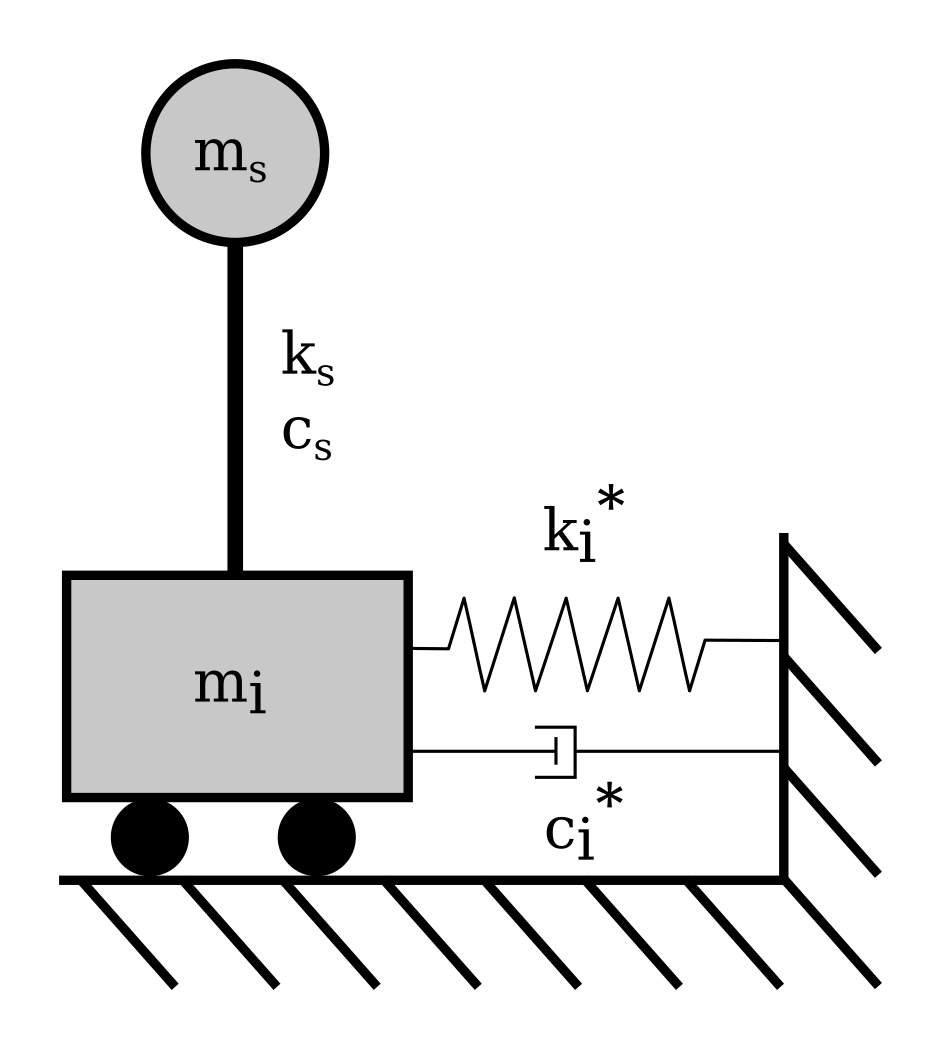
\includegraphics[width=0.5\textwidth]{voigt-kelvin-model.png}
    \caption{Voigt-Kelvin-Modell}
    \label{fig:vkm}
\end{figure}

\section{Ansatz über die Übertragsfunktion}
\label{sec:ansatzfunktion}

Im ersten Ansatz wurde die Möglichkeit untersucht, das Modell in zwei getrennte Systeme zu zerlegen und getrennt zu betrachten.
Die Annahme war, dass der Isolator lediglich als Filter auf das Antwortspektrum wirkt.

\begin{figure}[H]
    \centering
    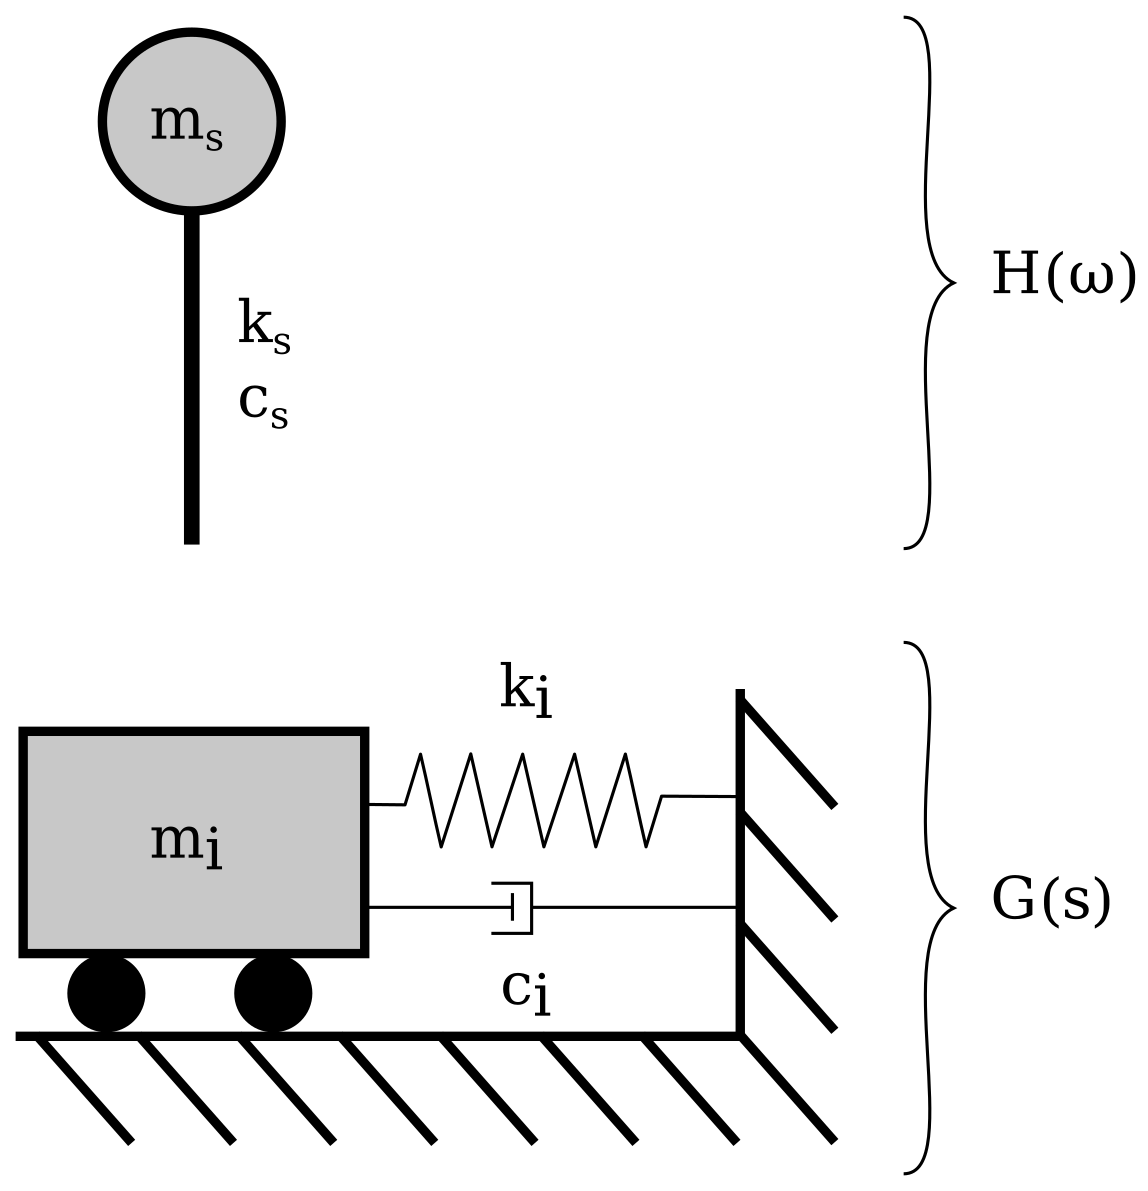
\includegraphics[width=0.7\textwidth]{composition.png}
    \caption{Komposition}
    \label{fig:composition}
\end{figure}

Die Funktion $H(\omega)$ stellt hier das Antwortspektrum dar und $G(s)$ die Übertragungsfunktion des Isolators.
Sie kann mittels der Laplace-Transformation

\begin{equation} \label{laplace}
F(s) = \int_{0}^{\infty} f(t)e^{-st}dt
\end{equation}

aus der Bewegungsgleichung des Isolators \cite{Kramer}

\begin{equation}\label{eq:bewegungsgleichung}
c_i \cdot \dot x(t) + k_i \cdot x(t) = - m_i \cdot \ddot x(t)
\end{equation}

für eine Kraftanregung zu

\begin{equation} \label{laplace2}
G(s)=\frac{X(s)}{F(s)} = \frac{1}{m_i \cdot s^2 + c_i \cdot s + k_i}
\end{equation}

bestimmt (wobei $s = i \omega$) und das isolierte Antwortspektrum ($H(\omega) \cdot |G(s)|$) gewonnen werden, da der Betrag der Übertragungsfunktion den Amplitudengang angibt.

Allerdings war dieser Ansatz nicht zielführend, da (wie an den Bewegungsdifferentialgleichungen (\cref{eq:BewegDGL1} und \cref{eq:BewegDGL2}) erkennbar ist) die Systeme gekoppelt sind und nicht getrennt betrachtet werden können.

\section{Vereinfachter Ansatz}
\label{sec:ansatzvereinfacht}

Zur Ermittelung der Eigenkreisfrequenzen des Zweimassenschwingers $\omega_{L,1,2}$ werden die Verhältniswerte

\begin{align}
\alpha &= \frac{k_2}{k_1} & \beta  &= \frac{m_2}{m_1} \\
\end{align}

eingeführt. Damit lassen sich die Eigenkreisfrequenzen und Perioden des isolierten Systems bezogen auf die Eigenkreisfrequenz $\omega$ des nicht isolierten Bauwerks wie folgt berechnen \cite{Pocanschi} \cite{Isemann}

\begin{align}
\omega_{L,1}^2 &= \frac{1 + \alpha + \beta - \sqrt{(1 + \alpha + \beta)^2 - 4 \alpha \beta}}{2 \beta} \omega^2\\
\omega_{L,2}^2 &= \frac{1 + \alpha + \beta + \sqrt{(1 + \alpha + \beta)^2 - 4 \alpha \beta}}{2 \beta} \omega^2
\end{align}

\begin{align}
T_{L,1} &= \frac{2 \pi}{\omega_{L,1}} & T_{L,2} &= \frac{2 \pi}{\omega_{L,2}}
\end{align}

Die Komponenten der Eigenvektoren $\vec{\Phi}_{1,2}$ lassen sich über die Beiwerte $\alpha$ und $\beta$ bestimmen.

\begin{align}
r_1 &= \frac{1 + \alpha - \beta + \sqrt{(1 + \alpha + \beta)^2 - 4 \alpha \beta}}{2}\\
r_2 &= \frac{1 + \alpha - \beta - \sqrt{(1 + \alpha + \beta)^2 - 4 \alpha \beta}}{2}
\end{align}

Die Schwingungsformen lauten damit wie folgt und können normiert werden.

\begin{align}
\vec{\Phi}_1 &= \binom{1}{r_1} & \vec{\Phi}_2 &= \binom{1}{r_2}\\
\vec{\Phi}_1 &= \binom{1/r_1}{1} & \vec{\Phi}_2 &= \binom{1/r_1}{1}
\end{align}

Der Beteiligunsfaktor der ersten Schwinungsform wird wie folgt definiert.

\begin{equation}
L_1 = \frac{\vec{\Phi}_1^T M \vec{I}}{\vec{\Phi}_1^T M \vec{\Phi}_1}
\end{equation}

Da die Steifigkeit des Isolators idealerweise deutlich geringer als die der Struktur ist gilt $\alpha \rightarrow 0$, $\vec{I} = \binom{1}{1}$ und $L_2$ wird klein, da die Schwingungsform durch die erste bestimmt wird.
Damit lässt sich die maximale absolute Beschleunigung der Massen der ersten Schwingungsform des Zweimassenschwingers infolge einer Fußpunktanregung bestimmen.

\begin{equation}
\ddot U_{max} = \vec{\Phi}_1 L_1 S_a(T_{L,1}, \xi_{L,1})
\end{equation}

Für die Erzeugung des isolierten Antwortspektrums wird die Steifigkeit der Struktur variiert und die Eigenkreisfrequenz dieser ermittelt.

\begin{equation}
k_{1,i} = \frac{4 \pi^2 m_1}{T_i^2}
\end{equation}

\begin{equation}
\omega = \sqrt{\frac{k_1}{m_1}}
\end{equation}

Da die Antwortspektren im Eurocode auf eine Dämpfung von 5\% normiert sind, wird unter der Annahme, dass die Dämpfung des Isolators dominiert, das Antwortspektrum abgemindert.

\begin{equation}\label{eta}
\eta = \sqrt{\frac{10}{5 + \xi_2}}
\end{equation}

\section{Ansatz über die Transmissibilität}
\label{sec:ansatztrasnm}

Die Beschleunigung aus dem Antwortspektrum wird in eine äquivalente harmonische Beschleunigungsanregung am Fußpunkt umgerechnet.
Anschließend wird über die Bewegungsgleichungen (\cref{eq:2DOF1,eq:2DOF2}) das Verhältnis der Amplituden von Fußpunktanregung zu harmonischer Schwingung an der oberen Masse $m_1$ hergeleitet.
Da die Perioden im Antwortspektrum die Eigenfrequenz des zur Erzeugung verwendeten Einmassenschwingers darstellen, kann eine harmonische Anregung erzeugt werden, deren Erregerfrequenz der Eigenfrequenz des Einmassenschwingers entspricht.
Zur Erzeugung eines isolierten Antwortspektrums soll dann die Steifigkeit $k_1$ variiert werden, sodass die Eigenfrequenz des oberen Systems der Periode des Antwortspektrums entspricht, und die Parameter des Isolators konstant bleiben.
So kann ein Isolationsspektrum erzeugt werden, das für jede Periode der aufgehenden Struktur eine äquivalente Beschleunigungsantwort angibt.

\subsection{Transmissibilität}
\label{sec:transm}

Die Bewegungsdifferentialgleichungen für das in \cref{fig:vkm} dargestellte System lauten:

\begin{align}
\ddot x_1 m_1 &= -(x_1 - x_2) k_1 -(\dot x_1 - \dot x_2) c_1 \label{eq:BewegDGL1}\\
\ddot x_2 m_2 &= (x_1 - x_2) k_1 + (\dot x_1 - \dot x_2) c_1 - (x_2 - x_3) k_2 - (\dot x_2 - \dot x_3) c_2 \label{eq:BewegDGL2}
\end{align}

Ansatz für harmonische Schwingung:

\begin{align*}
x_j &= S_j e^{i \omega t} & \dot x_j &= i \omega S_j e^{i \omega t} & \ddot x_j &= - \omega^2 S_j e^{i \omega t}
\end{align*}

\begin{align}
- \omega^2 S_1 m_1 e^{i \omega t} &= - (S_1 - S_2) e^{i \omega t} k_1 - (S_1 - S_2) i \omega c_1 e^{i \omega t} \label{eq:2DOF1} \\
- \omega^2 S_2 m_2 e^{i \omega t} &= (S_1 - S_2)(k_1 + i \omega c_1) e^{i \omega t} - (S_2 - S_3)(k_2 + i \omega c_2) e^{i \omega t} \label{eq:2DOF2}
\end{align}

\cref{eq:2DOF1} nach $S_2$ umgestellt:

\begin{align*}
\omega^2 S_1 m_1 &= (S_1 - S_2)(k_1 + i \omega c_1) \\
&\Rightarrow X_1 = \frac{\omega^2 m_1}{k_1 + i \omega c_1}\\
S_2 &= S_1 (1 - X_1)
\intertext{$S_2$ in \cref{eq:2DOF2} eingesetzt:}
\omega^2 m_2 S_1 &= - (S_1 - S_1 (1 - X_1)) (k_1 + i \omega c_1) + (S_1 (1 - X_1) - S_3) (k_2 + i \omega c_2)\\
&\Rightarrow X_2 = \frac{\omega^2 m_2}{k_2 + i \omega c_2}\\
S_1 (1 - X_1) X_2 &= S_1 (1-X_1) - S_3 - S_1 X_1 \frac{k_1 + i \omega c_1}{k_2 + i \omega c_2}\\
&\Rightarrow X_{12} = \frac{\omega^2 m_1}{k_2 + i \omega c_2}\\
S_1 (1 - X_1)(X_2 - 1) &= S_3 + S_1 X_{12}\\
S_3 &= S_1 [(1 - X_1)(1 - X_2) - X_{12}]
\end{align*}

Mit den komplexwertigen Transmissionskoeffizienten $X_1$, $X_2$ und $X_{12}$ ergibt sich die Transmissibilität aus dem Betrag des Verhältnisses von $S_1$ zu $S_3$.

\begin{equation}\label{eq:VT2DOF}
VT = \left\lvert \frac{S_1}{S_3} \right\rvert = \left\lvert \frac{1}{[(1 - X_1)(1 - X_2) - X_{12}]} \right\rvert
\end{equation}

Ein Hindernis stellen jedoch noch die Dämpfungsbeiwerte $c_1$ und $c_2$ dar.
Ein Ansatz, der hier untersucht werden soll, ist die steifigkeits- und massenproportionale modale Dämpfung. Sie wird auch als Rayleigh-Dämpfung bezeichnet. \cite{Pocanschi}

\subsection{Rayleigh-Dämpfung}
\label{sec:rayleigh}

Bei diesem Ansatz soll eine Proportionalität zwischen der Dämpfungsmatrix $C$ und den generalisierten Massen- und Steifigkeitsmatrizen $M^*$ und $K^*$ verwendet werden.

\begin{equation*}
C^* = \alpha M^* + \beta K^*
\end{equation*}

Wobei $\alpha$ und $\beta$ die Beiwerte der Rayleigh-Dämpfung sind.
$\alpha M$ kann als äußere und der Term $\beta K$ als innere Dämpfung verstanden werden.

Die Bestimmungsgleichungen der Beweirte lauten wie folgt. \cite{Shambhu}

\begin{align*}
\alpha &= \frac{2 \omega_1^* \omega_2^* (\xi_2 \omega_2^* - \xi_1 \omega_1^*)}{\omega_2^{*2} - \omega_1^{*2}}\\
\beta  &= \frac{2 (\xi_1 \omega_2^* - \xi_2 \omega_1^*)}{\omega_2^{*2} - \omega_1^{*2}}
\end{align*}

Um die Eigenkreisfrequenzen $\omega_1^*$ und $\omega_2^*$ zu erhalten, werden zunächst die Eigenkreisfrequenzen am ungedämpften System berechnet und die Eigenvektoren der zugehörigen Eigenformen bestimmt.

Eigenkreisfrequenz des ungedämpften Systems:

\begin{equation*}
\omega_{1,2}^2 = \frac{(k_2 + k_1) m_1 + k_1 m_2 \pm \sqrt{((k_2 + k_1) m_1 + k_1 m_2)^2 - 4 m_2 m_1 k_2 k_1}}{2 m_2 m_1}
\end{equation*}

Eigenvektoren des ungedämpften Systems:

\begin{align*}
\vec{\Phi}_1 &= \binom{\varphi_{11}}{\varphi_{21}} = \binom{1}{\varepsilon_1} & \vec{\Phi}_2 &= \binom{\varphi_{12}}{\varphi_{22}} = \binom{1}{\varepsilon_2}\\
\intertext{mit}
\varepsilon_1 &= \frac{k_2 + k_1 - m_2 \omega_1^2}{k_1} & \varepsilon_2 &= \frac{k_2 + k_1 - m_2 \omega_2^2}{k_1}
\end{align*}

Nach Betragsgröße normierte Eigenvektoren des ungedämpften Systems:

\begin{align*}
\varphi_{11} &= \sqrt{\frac{1}{1 + \varepsilon_1^2}}  &  \varphi_{12} &= \sqrt{\frac{1}{1 + \varepsilon_2^2}}\\
\varphi_{21} &= \varepsilon_1 \varphi_{11}            &  \varphi_{22} &= \varepsilon_2 \varphi_{12}
\end{align*}

Mit Hilfe der Eigenvektoren können die generalisierten Massen und Steifigkeiten ermittelt werden und damit die Eigenkreisfrequenzen.

Generalisierte Massen:

\begin{align*}
m_2^* &= \vec{\Phi}_1^T M \vec{\Phi}_1               &   m_1^* &= \vec{\Phi}_2^T M \vec{\Phi}_2\\
      &= \varphi_{11}^2 m_2 + \varphi_{21}^2 m_1     &         &= \varphi_{12}^2 m_2 + \varphi_{22}^2 m_1
\end{align*}

Generalisierte Steifigkeiten:

\begin{align*}
k_2^* &= \vec{\Phi}_1^T K \vec{\Phi}_1                                                          &   k_1^* &= \vec{\Phi}_2^T K \vec{\Phi}_2\\
      &= \varphi_{11}^2 (k_2 + k_1) - 2 \varphi_{21} \varphi_{11} k_1 + \varphi_{21}^2 k_1      &         &= \varphi_{12}^2 (k_2 + k_1) - 2 \varphi_{22} \varphi_{12} k_1 + \varphi_{22}^2 k_1
\end{align*}

Eigenkreisfrequenzen der zwei Einmassenschwinger:

\begin{align*}
\omega_1^* &= \sqrt{\frac{k_2^*}{m_2^*}}  &  \omega_2^* &= \sqrt{\frac{k_1^*}{m_1^*}}
\end{align*}

Damit ergeben sich die Dämpfungsbeiwerte der Rayleigh-Dämpfung

\begin{align*}
c_1^* &= \alpha m_1^* + \beta k_1^*\\
c_2^* &= \alpha m_2^* + \beta k_2^*
\end{align*}

und die gedämpfte Eigenfrequenz der ersten, durch den Isolator gesteuerten, Eigenform  

\begin{align*}
\omega_{1d} &= \omega_1 \sqrt{1 - \xi_2^2}\\
T_1         &= \frac{2 \pi}{\omega_{1d}} 
\end{align*}

Das System wird nun aus der Modal- zurück in die Normalform transformiert um die Dämpfungsmatrix $C$ zu erhalten. \cite{Rayleigh}

\begin{equation*}
C = \vec{\Phi}^{-T} C^* \vec{\Phi}^{-1}
\end{equation*}

Die Transmissibilität kann damit bestimmt werden.

\begin{equation}
VT(m_2, k_2, c_2, m_1, k_1, c_1)
\end{equation}

\subsection{Erzeugung des isolierten Antwortspektrums}
\label{sec:transmAWS}

Das isolierte Antwortspektrum kann aus dem elastischen Antwortspektrum erlangt werden.
Für jede Periode $T_i$ wird die Steifigkeit der aufgehenden Struktur berechnet, wobei die restlichen Parameter konstant bleiben.

\begin{equation}
k_{1,i} = m_1 (\frac{2 \pi}{T_i})^2
\end{equation}
  
Damit können die Transmissibilität $VT$, die gedämpfte erste Eigenkreisfrequenz $\omega_{1d}$

\begin{align}
\omega_{1d} &= \omega_1 \sqrt{1 - \xi_2^2} \\
T_1 &= \frac{2 \pi}{\omega_{1d}}
\end{align}

und die zugehörige äquivalente Amplitude der Beschleunigung der Fußpunktanregung

\begin{equation}
S_{a,x_3} = Sa(T_1)
\end{equation}

ermittelt werden. Die Ordinate des isolierten Antwortspektrums beträgt dann

\begin{equation}
S_{a,isoliert} = S_{a,x_3} \cdot VT
\end{equation}
  
\pagebreak
